\section{Stepper motors}
\label{sec:steppers}
This section gives a brief introduction into stepper motors and their control.
First, stepper motors and their types are described.
Then, a comparison of stepper driver ICs is given and some of the motion control technologies by Trinamic are described.

Stepper motors are a type of DC motors which move in discrete steps\cite{noauthor_all_nodate,noauthor_stepper_nodate}.
Such movement is achieved by their construction - they consist of a stator and a rotor, where the stator is made of coils
(two coils form a phase) wound on ridges, whereas the rotor consists is a ferromagnetic structure - either a permanent
magnet or a variable reluctance iron core\cite{noauthor_stepper_nodate}.

\subsection{Working principle}
\label{subsec:stepper_working_principle}
The basic working principle of stepper motors can be seen in the~Figure~\ref{fig:stepper_working_principle}.
In the Figure, we can see a three-phase bidirectional stepper motor.
First, the coils of the stator winding \textbf{A} are energized, which causes the ferromagnetic rotor to align with the magnetic field induced by the phase winding.
In the second step, the winding \textbf{B} is energized, causing the rotor magnetic field to realign with the newly induced magnetic field of the second winding.
This causes the motor to move.
In the next step, the winding \textbf{C} is energized, which again causes realignment of the rotor.
In the following steps, the coils are energized again but with different polarity making the rotor make a full turn.

\begin{figure}[H]
    \centering
    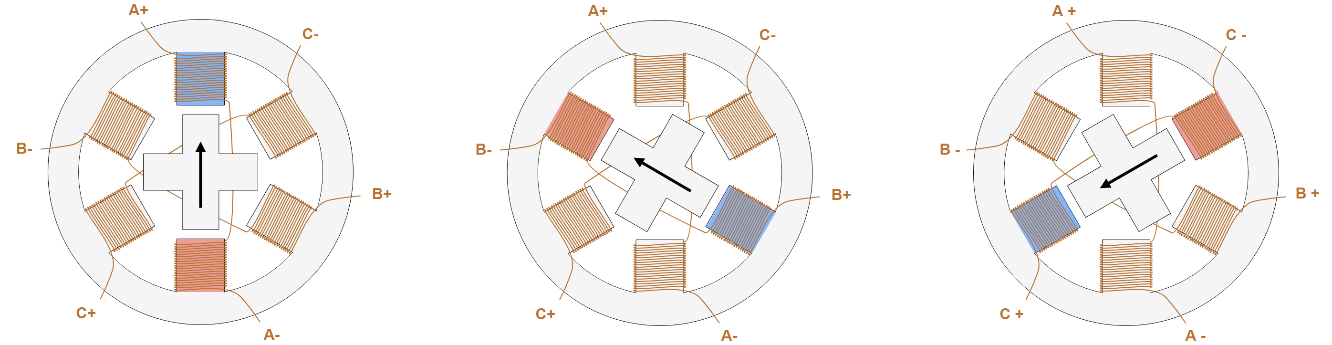
\includegraphics[width=\textwidth]{obrazky/stepper_principle}
    \caption{Working principle of a stepper motor~\cite{noauthor_stepper_nodate}.}
    \label{fig:stepper_working_principle}
\end{figure}

\subsection{Rotor}
\label{subsec:rotor}
There are three different constructions of rotors~\cite{noauthor_stepper_nodate}:
\begin{itemize}
    \item \textbf{Permanent magnet rotor} - utilizes a permanent magnet in the place of the stator.
    An advantage of this type of stator is good torque and also detent torque (the resistance of the motor shaft when no windings are energized)~\cite{noauthor_stepper_nodate}.
    \item \textbf{Variable reluctance rotor} - the rotor consists of a shaped iron core.
    The torques are generally lower and there is no detent torque~\cite{noauthor_stepper_nodate}.
    \item \textbf{Hybrid motor} - is created by combining a permanent magnet rotor with a variable reluctance rotor.
    There are two magnetic caps with teeths on top of each other that have an angular shift between them.
    The rotor is magnetized axially~\cite{noauthor_stepper_nodate}.
\end{itemize}

\subsection{Stator}
\label{subsec:stator}
The construction of stator depends on the number of phases the motor has.
Every phase consists of two windings and the windings can be center-tapped or not, which determines if the motor is bipolar or unipolar.
With unipolar windings, the center tapped lead is connected to the input voltage and the direction of the magnetic field is controlled by connecting ground to the other leads.
Bipolar motors do not have center tapped lead and the coil itself is controlled using a H-bridge.

\subsection{Phase Winding Energizing Techniques}
\label{subsec:winding_tech}
The way of energizing windings described in the Subsection~\ref{subsec:stepper_working_principle} is only one of four ways of controlling the windings.
This technique, where only one of the phases is energized at a time is called the wave mode.
it was described in detail in the Subsection~\ref{subsec:stepper_working_principle} and the sequence of energizing windings can be seen in the Figure~\ref{fig:stepper_wave_mode}.

\begin{figure}[H]
    \centering
    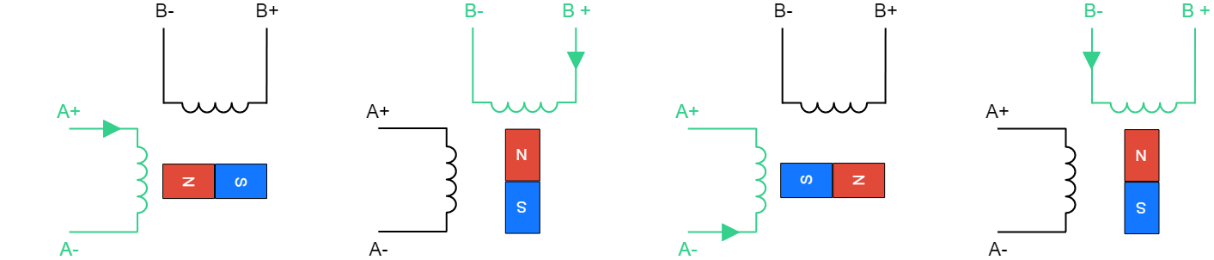
\includegraphics[width=\textwidth]{obrazky/wave_principle}
    \caption{Controlling stepper motor phase windings in wave mode~\cite{noauthor_stepper_nodate}.}
    \label{fig:stepper_wave_mode}
\end{figure}

\newpage
Another way of driving the motor is called the full-step mode.
In this mode, two phase windings are energized at the same time.
Changing the current direction in the winding causes the rotor to realign.
The advantage of this mode is higher torque as the magnetic field is stronger when the two of the phase windings are energized.
The working principle can be seen graphically in the Figure~\ref{fig:stepper_full_step_mode}.

\begin{figure}[H]
    \centering
    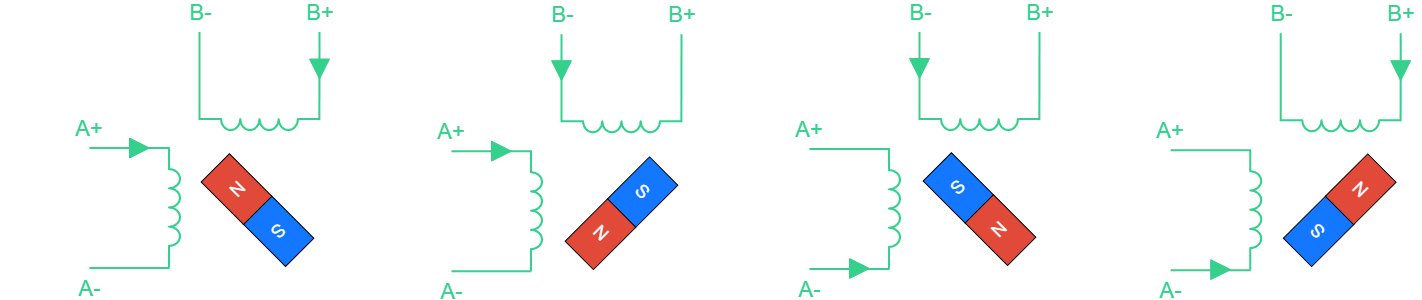
\includegraphics[width=\textwidth]{obrazky/full_step_principle}
    \caption{Controlling stepper motor phase windings in full step mode~\cite{noauthor_stepper_nodate}.}
    \label{fig:stepper_full_step_mode}
\end{figure}

Combining the wave mode and the full step mode results in a half-step mode.
In contrast to the previous driving modes, the step size of this mode is the half of the previous mode - in case of this virtual motor with permanent magnet motor 90\textdegree, therefore 45\textdegree.
This mode alternates between energizing only one phase winding and energizing both phase windings.
The disadvantage of this mode is that the produced torque is not constant as the torque is different when both phase windings are energized and when only one of them is.
The working principle can be seen in the Figure~\ref{fig:stepper_half_step_mode}.

\begin{figure}[H]
    \centering
    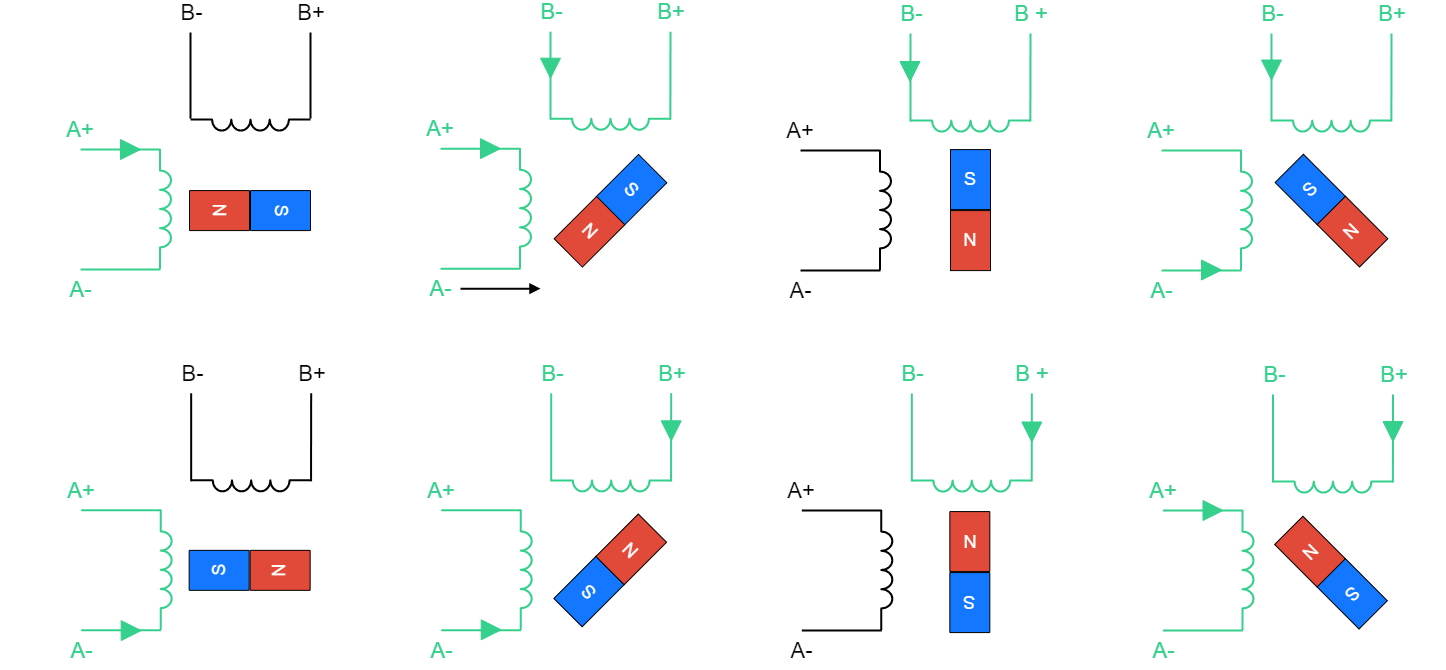
\includegraphics[width=\textwidth]{obrazky/half_step_principle}
    \caption{Controlling stepper motor phase windings in half step mode~\cite{noauthor_stepper_nodate}.}
    \label{fig:stepper_half_step_mode}
\end{figure}

The last technique for driving stepper motors is microstepping.
The advantage of this mode is that it reduces step size and has constant torque output~\cite{noauthor_stepper_nodate}.
The working principle for this mode is that the current flowing through the phase winding is controlled in some ratio, finely positioning the rotor as can be seen in the Figure~\ref{fig:microstepping}.
Microstepping is nowadays the prevalent way of stepper motor control as it allows for precision control and allows for constant torque.

\begin{figure}[H]
    \centering
    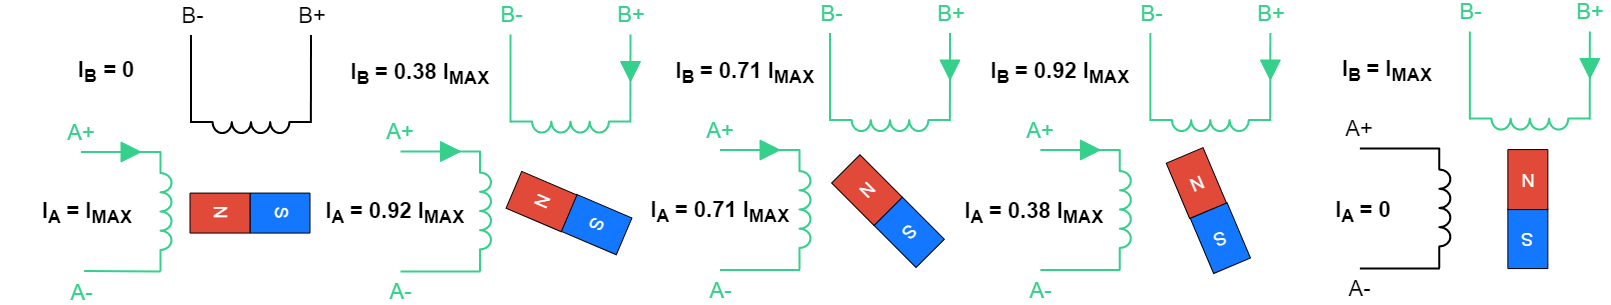
\includegraphics[width=\textwidth]{obrazky/microstepping}
    \caption{Controlling stepper motor phase windings in microstepping mode~\cite{noauthor_stepper_nodate}.}
    \label{fig:microstepping}
\end{figure}


\subsection{Stepper motor driver IC comparison}
\label{subsec:stepper_ic}
In order to select a proper driver IC for the SM4 stepper motor controller a simplified comparison was performed.
The resulting comparison can be seen in the following table:

% FIXME add info on the 2130 and 2209
\begin{sidewaystable}
    \centering
    \begin{tabular}{ |p{2cm}|p{2cm}|p{2cm}|p{2cm}|p{2.5cm}|p{2.5cm}|p{2cm}|p{4cm}| }
        \hline
        Name & Operating Voltage & Maximum current & Control Interface & Configuration Interface & Microstepping & Package & Advanced Features \\
        \hline
        \hline
        DRV8825 & 8.2-45~V & max 2.5~A (properly cooled, at 24~V, 25~\textdegree) & STEP/DIR & GPIO & up to 32 &  & None \\
        \hline
        A4988 & max 35~V & max 2 A & STEP/DIR & GPIO & up to 16 &  & None \\
        \hline
        TMC2100 & max 46~V & max 2 A (2.5 A peaks, properly cooled) & STEP/DIR & GPIO & up to 256 &  & MicroPlyer, SpreadCycle, StealthChop \\
        \hline
        TMC2130 & max 46~V & max 2 A (2.5 A peaks, properly cooled) & STEP/DIR & GPIO & up to 256 &  & MicroPlyer, SpreadCycle, StealthChop \\
        \hline
        TMC2209 & max 29~V & max 2 A (2.8 A peaks) & STEP/DIR & UART & up to 256 & & MicroPlyer, SpreadCycle, StealthChop2, CoolStep, StallGuard4 \\
        \hline
        TMC2226 & max 29~V & max 2 A (2.8 A peaks) & STEP/DIR & UART & up to 256 & & MicroPlyer, SpreadCycle, StealthChop2, CoolStep, StallGuard4 \\
        \hline
    \end{tabular}
    \caption{Comparison of stepper motor driver ICs}
    \label{tab:driver_ic_comparison}
\end{sidewaystable}
\newpage
\subsection{Trinamic motion control technologies}
\label{subsec:trinamic_tech}

